\chapter{Background} \label{chap_background}

In order to be able to accelerate a system, it is important to understand the mathematical model behind it. For this reason, we have included Section \ref{sec_ann} and \ref{sec_cnn}  from our previous work \cite{Halvorsen2014}, which purposed a theoretical accelerator architecture. The sections will introduce the fundamental mathematics and concepts behind the \textit{Convolutional Neural Network} (CNN) model. They give a basic introduction to both general neural networks and \textit{CNNs}. Section \ref{sec_zedboard} will present the hardware platform we used to implement our accelerator. 

\section{Artificial Neural Networks}\label{sec_ann}

An \textit{Artificial Neural Network} (ANN) \cite{Minsky1969}\cite{Bishop2006} is a computational model that is used for machine learning and pattern recognition. The name and basic concept is inspired by how the animal brain uses a network of neurons to recognize and classify objects. Depending on the input, different neurons \textit{activate} (or \textit{fire}), making the brain able to decide what kind of pattern it is detecting. 

An ANN can intuitively be viewed as a probabilistic classifier. Depending on the input data, it will calculate the probability that the data belongs to a certain \textit{class} (e.g. an object in an image or an investment decision). The network can be trained to recognize different classes by being provided a set of labeled training data, e.g. a set of faces and a set of non-faces. It can then learn to decide whether an image contains a face or not. This is called supervised learning. The network can also be trained unsupervised, by providing it with a set of unlabeled images. The latter technique is used to find hidden structures in the data, by learning the network to recreate the input. But for this project only supervised learning is relevant.  

\subsection{Definition} \hfill \break
An ANN  consists of a number of layers containing a set of so-called \textit{neurons} (see Figure \ref{fig_neuron}), also known as \textit{units}. A neuron takes in a set of values as input (e.g. image pixels), where each value is associated with a respective weight. The input and the weights are multiplied and summed, and the result is used to calculate a non-linear \textit{activation function}. Formally a neuron's input and output is defined as:


\begin{equation}\label{eq_neuron_in}
Input: \{x_1, x_2,\dots, x_n\} = \mathbf{x} 
\end{equation}

\begin{equation}\label{eq_neuron_out}
Output: f(\mathbf{w^{T}x)} = f(\sum_{i=1}^{n}w_i x_i + b) = o
\end{equation}

Where \textbf{w} is the vector containing connection weights and b is the neuron bias. \textit{f(...)} is the activation function, which eumulates the activation of a neuron in the brain, i.e. it decides whether the neuron is on or off. It also causes the values in the network to have a reasonable value interval. \textit{f(...)} tends to be either:

\begin{equation}
Sigmoid: f(z) = \frac{1}{1 + e^{-z}}
\end{equation}



\begin{equation}
\text{Hyperbolic tagent:} f(z) = tanh(z) = \frac{e^z - e^{-z}}{e^z + e^{-z}}
\end{equation}

The reason these functions are used is that they have the non-linear property, which increases the expressivness of the network. Thus reducing the number of neurons the network needs to solve a given problem. In addition both function have ranges [0, 1] and [-1, 1], respectively, which translates well into probability computation. I.e. you can view the value of the activation function as the probability of that neuron activating.  
 

\begin{figure}[h!]
  \centering
      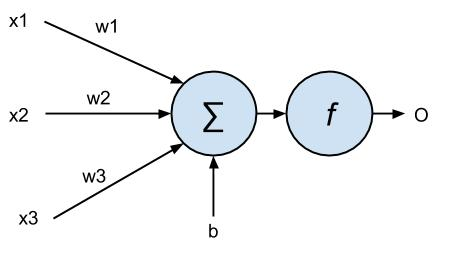
\includegraphics[width=0.5\textwidth, scale=0.1]{Figures/Background/Neuron}
  \caption[Neuron]{A single neuron with three inputs. }
  \label{fig_neuron}
\end{figure}

An ANN consist of $ n_l $ layers, each containing a set of neurons. The first layer is \textit{the input layer}, and the last layer is \textit{the output layer}. The layers in between are called \textit{the hidden layers}. Each layer uses the previous layer's output as input. The input layer is provided with the initial input and uses it to calculate the activation function for each of its neurons. The result is propagated to the first hidden layer, and continues up until it reaches the output layer, which provides the final output. This is known as a \textit{feedforward neural network.}

The network takes in two parameters: 

\begin{equation}
	(\mathbf{W, b}) = (\mathbf{W}^{(1)}, b^{(1)}, \mathbf{W}^{(2)}, b^{(2)}, \dots , \mathbf{W}^{(n_l)}, b^{(n_l)})	
\end{equation}
 Where \textbf{W} is a 3-dimensional matrix containing the weight matrix for each layer. $ \mathbf{W}^{(l)} $ contains the weight matrix for the weights going from layer \textit{l} to \textit{l+1}. E.g. in the case of Figure \ref{fig_ann}, $ \mathbf{W}^{(1)} \in \Re ^{3 \times 4}$ and $ \mathbf{W}^{(2)} \in \Re ^{4 \times 2}$.

\begin{figure}[h!]
  \centering
      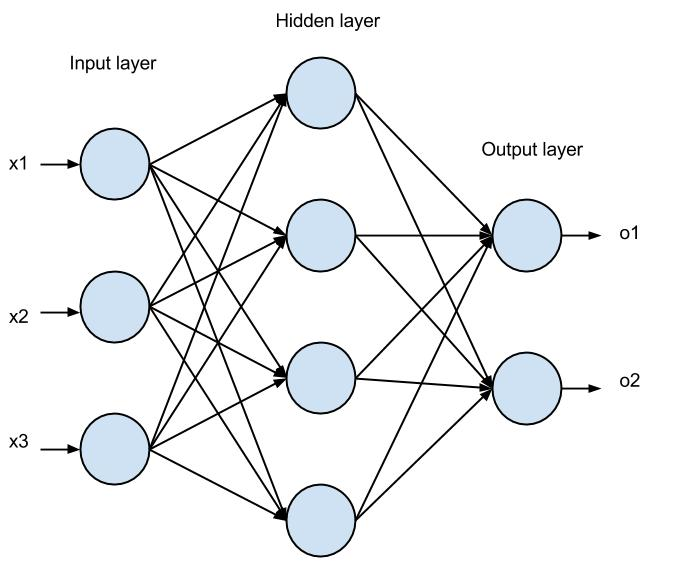
\includegraphics[width=0.5\textwidth]{Figures/Background/ann}
  \caption{An Artificial Neural Network.}
  \label{fig_ann}
\end{figure}


\subsection{Training} \label{sec_ann_training}
During the training of the network, it is the parameters $ (\mathbf{W, b}) $ that are altered in order to adapt the network to the training data. This is done by providing the network with a set of training samples, where an input and an expected output is provided. By using a cost function we can then figure out how we should tune our weights and biases in order to reduce the error rate. In other words, our goal is to minimize a cost function over a set of training samples. This can be done by using \textit{gradient descent} and the \textit{backpropagation algorithm} \cite{Rumelhart1986}\cite{Leonard1990}\cite{LeCun1998}. 

Let the cost function for a single training example $(x,y)$ be defined as:

\begin{equation}
	Cost(\mathbf{W},\mathbf{b}; x, y) = \frac{1}{2}(h_{\mathbf{W},\mathbf{b}}(x) - y)^2
\end{equation}

Where $ x $ is the input, $ h_{\mathbf{w},b}(x) $ is the actual output of our network and \textit{y} is the correct output.
Then the cost function for \textit{m} training examples $ ((x^{1}, y^{1}), (x^{2}, y^{2}), \dots, (x^{m}, y^{m})) $ is:

\begin{equation}
	Cost(\mathbf{W},\mathbf{b}) = \frac{1}{m}\sum_{i=1}^{m}Cost(\mathbf{W},\mathbf{b};x^{(i)},y^{(i)}) + \frac{\lambda}{2}
	\sum_{l=1}^{n_l-1}\sum_{i=1}^{s_l}\sum_{j=1}^{s_l+1}
	(\mathbf{w}_{ji}^{l})^2
\end{equation}
 
Where the first term is simply the average sum-of-squares error. The second term is the \textit{regularization term}, or \textit{weight decay term}, which tends to reduce \textit{overfitting}. ANNs have a vast number of parameters, i.e. weights, which makes it susceptible to random noise. This can greatly reduce the networks ability to provide correct predictions, but this  can be mended by the regularization term. 

Based on this we can use gradient descent to compute how we should alter the weights in order to reduce the cost function. One iteration of gradient descent updates \textbf{w} and \textit{b} as follows:

\begin{equation}
	w_{ij}^{(l)} = w_{ij}^{(l)} - \alpha\frac{\partial}{\partial w_{ij}^{(l)} }Cost(\mathbf{W},\mathbf{b})
\end{equation}

\begin{equation}
	b^{(l)} = b^{(l)} - \alpha\frac{\partial}{\partial b_{i}^{(l)} }Cost(\mathbf{W},\mathbf{b})
\end{equation}

Where $ \alpha $ is the learning rate, which is a predetermined constant. $ w_{ij}^l $ denotes the weight between neuron j in layer l, and neuron i in layer l+1. $ b_i^l $ denotes the bias associated with neuron \textit{i} in layer l+1. 

Note that this would only make us able to compute the gradient for the output layer. In order to perform gradient descent on the hidden layers, we need to propagate the error from the output layer backwards, to the hidden layers. For this we use the \textit{backpropagation algorithm}. Let $ o_i^{(l)} $ denote the output of the $i$th neuron in layer $l$, and $z_k^{(l)}$ is the weighted sum of the inputs plus the bias for the $k$th neuron in layer l. Then the \textit{backpropagation algorithm} can be formalized as follows: 

\begin{enumerate}
	\item Perform a feedforward pass, computing the output of every layer.
	\item For each output neuron k in the output layer, compute \textit{the error term}: 
	\begin{equation}
		\delta_k = \frac{\partial}{\partial z_{k}^{(n_l)} }Cost(\mathbf{W,b}; x, y) = -o_k^{n_l}(1-o_k^{n_l})(y_k-o_k^{n_l})
	\end{equation} 
	\item For each hidden layer $ l = n_l - 1, n_l - 2,\dots, 2 $ compute: 
	\begin{equation}
		\delta_i^{l} = o_i^l(1-o_i^l)\sum_{j=1}^{s_{l+1}} w_{ij}^l \delta_j^{l+1} 
	\end{equation}
	\item Compute the partial derivative for each weight and bias:
	\begin{equation}
		\frac{\partial}{\partial w_{ij}^{(l)} }Cost(\mathbf{W,b}; x, y) = o_j^{(l)}\delta_i^{(l+1)}
	\end{equation}
	
	\begin{equation}
		\frac{\partial}{\partial b^{(l)} }Cost(\mathbf{W,b}; x, y) = \delta_i^{(l+1)}
	\end{equation}
\end{enumerate}
	
Now, combining \textit{gradient descent} and the \textit{backpropagation algorithm} we can describe an algorithm to train our network: 

\begin{enumerate}
	\item Initialize the weights $ \mathbf{w}^{(l)} $ and $ b^{l} $ to random values for every layer \textit{l}.
	\item Do steps 3 to 5 until the $ Cost(\mathbf{W, b}) $ function is low enough or converges. This is referred to as an \textit{epoch}. 
	\item Set $ \Delta\mathbf{w}^{(l)} := 0 $ and $ \Delta b^{(l)} := 0 $ for all \textit{l}.
	\item For i = 1 to m,
		\begin{enumerate}
			\item Use the backpropagation algorithm to compute $ \nabla_\mathbf{w^{(l)}}Cost(\mathbf{W, b};x^{(i)},y^{(i)}) $ and $ \nabla_b^{(l)}Cost(\mathbf{W, b};x^{(i)},y^{(i)}) $ for every layer \textit{l}.
			\item  Set $ \Delta\mathbf{w}^{(l)} := \Delta\mathbf{w}^{(l)} + \nabla_\mathbf{w^{(l)}}Cost(\mathbf{W, b};x^{(i)},y^{(i)}) $. 
			\item  Set $ \Delta b^{(l)} := \Delta b^{(l)} + \nabla_{b^{(l)}}Cost(\mathbf{W, b};x^{(i)},y^{(i)}) $. 
		\end{enumerate}
	\item Update the parameters:
		\begin{equation*}
			\mathbf{w}^{(l)} = \mathbf{w}^{(l)} - \alpha[(\frac{1}{m}\Delta\mathbf{w}^{(l)}) + \lambda\mathbf{w}^{(l)}]
		\end{equation*}
		
		\begin{equation*}
			b^{(l)} = b^{(l)} - \alpha[\frac{1}{m}\Delta b^{(l)}]
		\end{equation*}
\end{enumerate}

\subsection{Issues with object recognition}\label{ann_issues}

While the ANN model have proven useful in several applications, it falls short when it comes to object recognition in images. According to \cite{LeCun1998} there are three major reasons for this: . 

\begin{enumerate}

	\item \textbf{Topology}. A fully connected ANN does not take into consideration the topology of the input. An image has a strong 2D spatial locality correlation, which makes it possible to combine low-order features (edges, end-points etc.) in the same area into higher-order features (noses, ears etc.).  
	
	\item \textbf{Scalability}. Even small images contains a large amount of pixels/inputs, e.g. a $ 32 \times 32 $ image contains 1024 pixels/inputs. A fully connected network with 100 hidden units would then end up with $ 1024 \times 100 $ weights that needs to be calculated in the first layer. Thus making it harder to scale for larger images and rather inefficient .
	
	\item \textbf{Object variance.}While objects are similar enough, on a higher level, to be grouped together into a class, they can still be very different on a lower level. E.g. a human face have several features that are needed for it to be defined as a face, e.g. eyes, mouth, nose etc. But the size and shape of these features tend to be very different from person to person. While it is possible for a standard ANN to compensate for these internal differences within a class, it would have to make three costly compensations. 1) The network would have to be very large, 2) it would probably contain several neurons with similar weight vectors positioned at different places in the network, and 3)  it would require a massive amount of training samples. 
	
\end{enumerate}



% % % % % % % % % % % % % % % % % % % % % % % % % % % % % % % % % % % %
%CONVNET!
% % % % % % % % % % % % % % % % % % % % % % % % % % % % % % % % % % % % 
\section{Convolutional Neural Network}\label{sec_cnn}

A \textit{Convolutional Neural Network} \cite{LeCun1998} (CNN) is an extension of the \textit{Artificial Neural Network} model, which is made specifically for object recognition in images or speech recognition. It was made in order to solve the issues that the classic ANN model faced. 


\begin{figure}[h!]
  \centering
      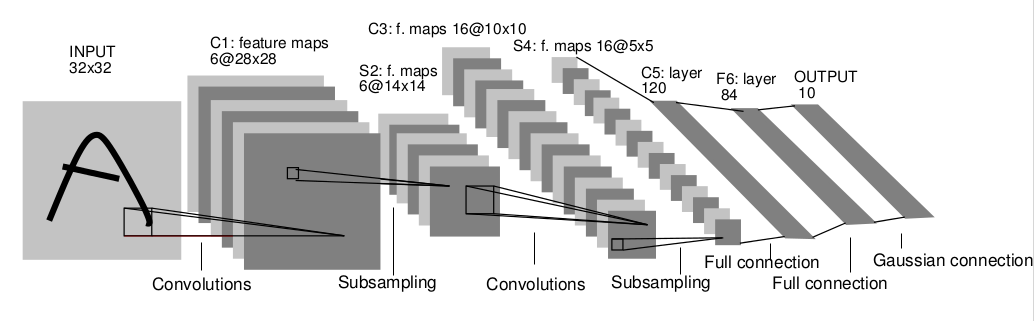
\includegraphics[width=1.2\textwidth]{Figures/Background/convnet}
  \caption[The LeNet-5]{An example CNN, the LeNet-5 \cite{LeCun1998}. It consists of two convolution and subsampling/pooling layer pairs, which are connected to a fully connected ANN with 10 output classes.}
  \label{fig_cnn}
\end{figure}

\subsection{Definition} \label{sec_cnn_def}

The CNN model adds two additional types of layers, in addition to the standard ANN layers: a \textit{convolution layer} and a \textit{subsampling/pooling layer}. The idea behind the two new layers is to exploit the local 2D structure of images, i.e. pixels close to each other are highly correlated. By using local correlation one can extract and combine small local features (e.g. edges, corners, points) into higher-order features (e.g. a nose, a mouth, a forehead), which can in the end be recognized as an object (e.g. a face).  A full network is illustrated in Figure \ref{fig_cnn}.


\paragraph{Convolution layer}  \hfill \break
The convolution layer extracts a set of features from a set of input images. For each feature, the respective feature is extracted from all the input images and put in a feature map. E.g. if the filter extracts vertical edges, only the vertical edges from all the input images would remain in the resulting feature map. Thus different features can be extracted by having several feature maps that extracts different features. 

The extraction is done by performing a \textit{convolution operation} on the image, using a \textit{kernel} that acts like a filter. The kernel is a 2D matrix that contains a set of weights. Depending on values of the weights, convoluting the image with the kernel will have wide range of effects, e.g. sharpening, bluring, edge detection  and feature extraction. By training our network we can configure the weights to extract the features we need in order to recognize our desired classes. 

After the convolution operation has been performed, a bias is added to every element in the feature map and the result is sent through a non-linear function, e.g. the hyperbolic tangent.

Formally we can define the convolution layer as follows. The layer accepts \textit{n} images $ X_1, X_2, \dots, X_n $ as inputs, and produces \textit{m} feature maps, $F_1, F_2, \dots, F_m $. These feature maps are produced using a set of \textit{m} learned kernels $ W_1, W_2, \dots, W_m $.  Each feature map $ F_t $ is then produced by computing:
 

\begin{equation}
\mathbf{F}_t = Tanh(b_t+\sum_{i=1}^{n}\mathbf{X}_i*\mathbf{W_t})
\end{equation}

Where \textbf{F} is the resulting feature map, X is the input image, \textbf{W} is the kernel matrix, and \textit{b} is the bias. $ X * W $ is the convolution operation, which is defined as:

\begin{equation}
y_{ij} = \sum_{q=1}^{k}\sum_{p=1}^{k} x_{i+q, j+p}w_{qp}
\end{equation}

Where $ x_{ij} $ is a value of the input matrix, $ w_{mn} $ is a value in the $ k \times k $ kernel matrix, and $ y_{ij} $ is a value of the output matrix.

E.g. consider the LeNet-5 in Figure \ref{fig_cnn}, in the first layer C1 the input is a single $ 32 \times 32 $ image which is convoluted with 6 kernels, producing 6 feature maps. Thus $ n = 1 $ and $ m = 6 $. The resulting feature maps are then further processed by a subsampling/pooling layer S2 (see next section), which are used as input to the next convolutional layer C3. The six processed feature maps are then convoluted with 16 kernels, producing 16 new feature maps. Thus in this layer $ n = 6 $ and $ m = 16 $. 



This helps solve the first two issues from Section \ref{ann_issues}. The neurons in a feature map share the same kernel, thus the same weights, which greatly reduces the size of the network. The convolution operation applies a 2D filter on the image, which makes the network able to exploit the spatial correlation in the image. 

\paragraph{Subsampling/pooling layer}  \hfill \break
Once a feature has been detected, the exact position become less important. For example, the distance between the mouth and the eyes tend to vary between persons. So in order to make the CNN not too sensitive to the relative placement of features, the accuracy of the all feature maps needs to be reduced. This can be done by subsampling (i.e. partitioning) the feature map into $ s \times s $ non-overlapping submatrices, and then perform a pooling operation on each respective matrix. There are two types of pooling operations which are used for CNNs: 

\begin{itemize}
	\item \textit{Max-pooling} extracts the maximum value of the submatrix.
	\item \textit{Average-pooling} extracts the average value of all the elements in the submatrix.
\end{itemize}

\begin{figure}[h!]
  \centering
      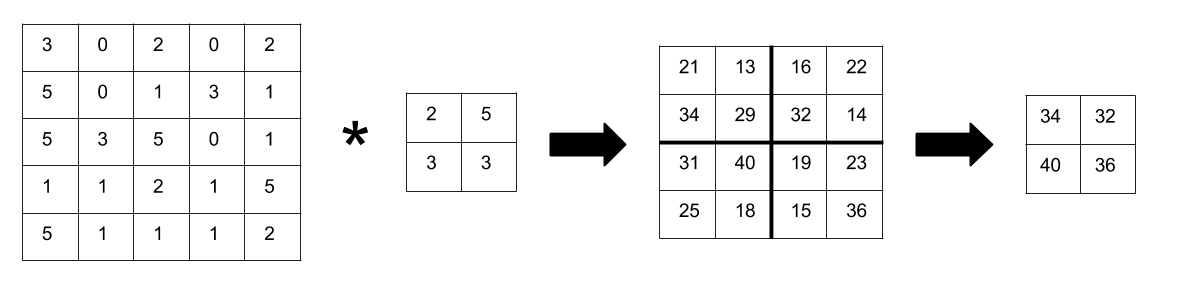
\includegraphics[width=1.0\textwidth]{Figures/Background/Convolution-Maxpooling}
  \caption[Convolution and subsampling/max-pooling operation]{Illustration of the convolution and subsampling/max-pooling operations. The leftmost matrix is convulted with a $ 2 \times 2 $ kernel, and the resulting matrix is subsampled into four non-overlapping areas where the max value is extracted.}
  \label{fig_conv_ss_mp}
\end{figure}

Given an output of \textit{m} feature map inputs, each output matrix can be defined as:

\begin{equation}
	\mathbf{O_t} = Tanh(b_{t} + subsample\_pool(\mathbf{F_t}))
\end{equation}


Where $O_t$ is the \textit{t}'th output matrix, $ b_t $ is \textit{t}'th bias, and $F_t$ is the \textit{t}'th input feature map, and the \textit{subsample\_pool()} function's operation is defined as either:

\begin{equation}
o_{ij} = max(x_{i \times s+p, j \times s+q}) \qquad\qquad q,p \in 1, 2, \dots, s
\end{equation}

or

\begin{equation}
o_{ij} = \frac{1}{c} \sum_{p=1}^{s}\sum_{q=1}^{s} x_{i+p, j+q}
\end{equation}

Where $ o_{ij} $ is a value in the output matrix and $ f_{ij} $ is a value in the feature map, c is a trained constant, and \textit{s} is the dimension of the subsampling size. A max-pooling operation is illustrated in Figure \ref{fig_conv_ss_mp}.

Thus, the subsample/pooling layer helps solve the two last issues from Section \ref{ann_issues}. By reducing the accuracy, the network is less sensitive to the difference between instances of a class. This also causes the network size to be smaller, since it does not require neurons to recognize the differences. 

Figure \ref{fig_conv_ss_mp} illustrates the convolution operation and the subsample/max-pooling operation, while Figure \ref{fig_visual_conv_ss_mp} illustrates the full operation of the convolution and subsampling/pooling layers. 

\begin{figure}[h!]
  \centering
      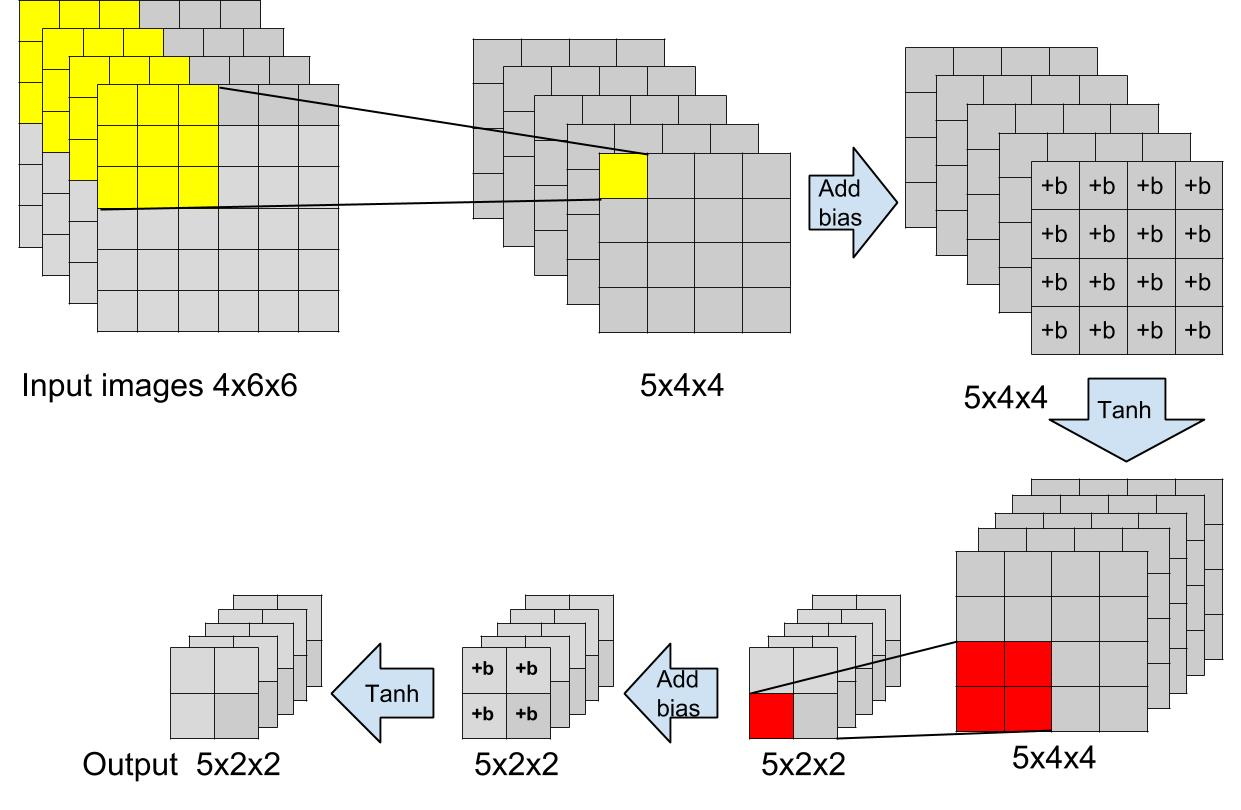
\includegraphics[width=1.0\textwidth]{Figures/Background/Convolution_subsample_pool}
  \caption[Convolutional layer operation]{A visual overview of the operations performed by the convolution layer and subsampling/pooling layer with four input images. Yellow represents the convolution operation, and red represents the subsampling/max-pooling operation.}
  \label{fig_visual_conv_ss_mp}
\end{figure}



\subsection{Training} \label{sec_cnn_training}
As mentioned, a CNN consists of three types of layers: a convolution layer, a subsampling/pooling layer and fully connected layer. The latter is trained as described in Section \ref{sec_ann_training}, using backpropagation and gradient descent. The two other layers use the same general algorithm, but the error $ \delta^l $ and the gradient of $ Cost(\mathbf{W,b}; x, y) $ is calculated differently. 

Since the backpropagation aglorithm starts at the last layer and work its way backwards, the error is first calculated for the fully connected layers. It is then provided to the subsampling/pooling layer, and finally to the convolution layer. Thus we first need to calculate the error for the subsampling/pooling layer, so we can propagate it to the convolution layer. 

The subsampling/pooling layer does not contain any weights, and can therefore not be tuned. Thus it only needs to propagate the error it receives. Depending on which pooling operation is used, there are two respective methods for this. For max pooling, the error is simply propagated to the neuron that was chosen as the maximum value, while the rest are set to zero. For average-pooling we have to distribute the error evenly between all the responsible neurons. We therefore define the function \textit{upsample(...)}, which performs the correct propagation operation depending on the type of pooler. 

We can now formally define how to calculate the error and the gradient by simply replacing the equations in step 3 and 4 in the backpropagation algorithm with the following equations. For simplicity we assume that convolution and subsampling/pooling is done in a single layer \textit{l}.




\begin{equation}
	\delta_{k}^{l} =  upsample( (\mathbf{W}_{k}^l)^T \mathbf{\delta}_{k}^{l+1})\bullet f'(\mathbf{Z}_k^l)
\end{equation}

Where $  (\mathbf{W}_{k}^l)^T $ is the weight matrix in layer \textit{l}, $  \mathbf{\delta}_{j}^{l+1} $ is the error matrix for layer $ l + 1 $, $ \bullet $ is the element-wise product (i.e. Hadamard product), $ f'(\mathbf{Z}_k^l) $ is the matrix containing the derivative of the activation function, and k indexes the filter number. I.e. it contains $ o_{kij}^l(1-o_{kij}^l) $ for every neuron at index \textit{ij} in feature map \textit{k} in layer \textit{l}. 

Using this we can calculate the gradient:

\begin{equation}
	\frac{\partial}{\partial \mathbf{w}_k^{(l)} }Cost(\mathbf{W,b}; x, y) = \sum_{i=1}^{m}(\mathbf{o}_i^{(l)})*\delta_k^{(l+1)}
\end{equation}

\begin{equation}
	\frac{\partial}{\partial b_k^{(l)} }Cost(\mathbf{W,b}; x, y) = \sum\delta_k^{(l+1)}
\end{equation}

\section{Potential for parallelism} \label{sec_pot_parallelism} 

A vast amount of the computation required by a CNN can be parallelized. Thus, in order to achieve the processing of the network it is important that these potential parallelizations are identified and exploited. The most obvious being:

\begin{enumerate}
    
    \item The convolution of a matrix $ n \times n $ using a $ k \times k $ kernel consists of $ (n - k + 1) \times (n - k + 1) $ convolution operation, which each can be done in parallel. Thus convoluting the whole matrix could potentially take only the time it takes to perform one convolution operation. 
    
    \item The subsampling/pooling operation can also be parallelized by pooling all of the individual submatrices at the same time.  
	
    \item The computation of each of the individual feature maps and their corresponding subsampling/pooling. Which \cite{Chakradhar2010} referred to as \textit{inter-parallelism}.
	
    \item It is also possible to parallelize the computation of the feature maps that take more than one matrix as input. This is the case in the subsequent layers after the first. Which \cite{Chakradhar2010} referred to as \textit{intra-parallelism}.
	
    \item The activation of each neuron in the fully connected layer. One option is to parallelize them by creating a binary tree multiplier, where you have \textit{n} units compute the product of the input and its respective weight, then you use $ \frac{n}{2} $ units to add two of the results each, and so on until you have a single value. This will reduce the time it takes from \textit{n} time to $ log_2 n $ time if they can all be done in parallel.   
\end{enumerate}


\section{ZedBoard} \label{sec_zedboard}

We choose the ZedBoard as the development board for our implementation of our accelerator prototype. It contains a \textit{Xilinx Zynq�-7000 All Programmable System-on-Chip (SoC)} Z-7020, which consists of a dual-core \textit{ARM Cortex-A9 MPCore based Processing System (PS)} and an Artix-7 XC7Z020 FPGA as \textit{programmable logic} (PL) \cite{zyng_resource_documentation}. The PS includes on-chip memory, external memory interfaces, and a number of I/O peripherals. The system offers the flexibility and scalability of an FPGA, while providing performance, power, and ease of use typically associated with ASIC and \textit{application specific standard product} (ASSP) \cite{zyng_documentation}.

The PL makes use of the second version of the \textit{Advanced eXtensible Interface} (AXI4) bus protocol, which is part of the \textit{ARM Advanced Microcontroller Bus Architecture} (AMBA) \cite{Axi4_doc}. There are three types of AXI4 interfaces:

\begin{itemize}
\item AXI4 - for high-performance memory-mapped requirements.
\item AXI4-Lite - for simple, low-throughput memory mapped communication.
\item AXI4-Stream - for high-speed streaming data.
\end{itemize}

As long as a component in the PL implements any of these interfaces, it can be connected directly to the PS through a set of AXI4 bus ports. For the rest of this report we will refer to AXI4-Lite as AXI, and AXI4-Stream as AXIS. The prefixes S\_ and M\_ will refer to slave and master port, respectively. These acronyms will be use extensively in Section \ref{sec_hardware_architecture}.

The feature that makes the ZedBoard especially well-fitted for hardware acceleration applications, is the tight coupling between the PS and the PL. The ARM processors can be connected directly to any component in the PL area through the \textit{extended multiplexed I/O} (EMIO) port or a set of general purpose AXI ports (see Figure \ref{fig_zynq_architecture}). In addition, there are four high performance (HP) AXI4 ports that PL components can use to access external memory directly. At max capacity the HP AXI4 ports have a bandwidth of 1200 MB/s. This integration of the PS with the PL allows levels of performance that the two-chip solutions (e.g. an ASSP with an FPGA) cannot match due to their limited I/O bandwidth, latency and power budgets \cite{zyng_documentation}.


% http://www.xilinx.com/support/documentation/data_sheets/ds190-Zynq-7000-Overview.pdf
% http://www.xilinx.com/publications/prod_mktg/zynq7000/Zynq-7000-combined-product-table.pdf
% http://www.xilinx.com/support/documentation/ip_documentation/axi_ref_guide/v13_4/ug761_axi_reference_guide.pdf


\begin{figure}[h!]
  \centering
      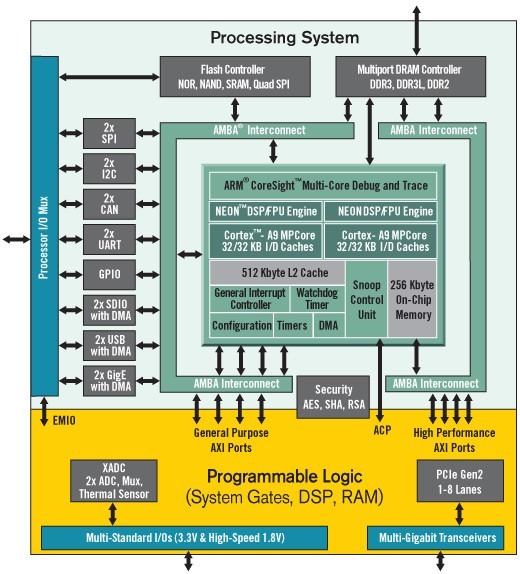
\includegraphics[width=1.0\textwidth]{Figures/Background/zynq_architecture}
  \caption[Zyng-7000 system architecture.]{Zyng-7000 system architecture.}
  \label{fig_zynq_architecture}
\end{figure}
